\section*{Introduction}

For most of the history of machine learning on tables, the honest recommendation has been gradient-boosted trees. Random forests, XGBoost, LightGBM, CatBoost and AutoML systems built on them handle mixed feature scales, missing values and nonlinear interactions with little tuning, and careful benchmarks have repeatedly found that deep networks struggle to beat them on medium-sized tabular data with many more rows than features.\citep{breiman2001random,chen2016xgboost,ke2017lightgbm,prokhorenkova2018catboost,erickson2020autogluon,grinsztajn2022tree}

Hollmann and colleagues challenged that recommendation with TabPFN, described in their title as giving ``accurate predictions on small data with a tabular foundation model''.\citep{hollmann2025accurate} TabPFN is a transformer pretrained on synthetic tables; at prediction time it reads the labeled training rows as context and returns predictions without fitting task-specific parameters. On 29 classification and 28 regression datasets of up to 10,000 rows and 500 features, the original study reported that it outperformed gradient-boosted baselines both at default settings and after up to four hours of tuning, taking seconds per dataset on a machine with a GPU. Later releases extended the supported data size, to 50,000 rows and 2,000 features for TabPFN-2.5 and to larger regimes for TabPFN-3,\citep{priorlabs2025tabpfn25,priorlabs2026tabpfn3} and Google's TabFM, described in an announcement and a software release, applies the same in-context principle with row-and-column attention and a synthetic prior built from structural causal models.\citep{google2026tabfm,tabfmsoftware2026} An independent comparison against tuned established methods on twelve binary clinical tasks found that TabPFN exceeded the best of them in 2 of 12 tasks, with most differences in AUROC within 0.02, although with predictors, endpoints and budgets that differ from ours.\citep{shaktah2026established}

Cancer multiomics is a natural, and demanding, place to reuse these models. Cohorts typically contain a few hundred patients and thousands of molecular features. Benchmarks of censored survival models on TCGA cohorts have found that a clinical-variables-only reference performs about as well as the best molecular models in aggregate, and that adding modalities does not reliably help.\citep{herrmann2021benchmark,li2024combining,wissel2023systematic} Cohorts also differ in prognosis, source and assay coverage, and TCGA molecular profiles are organized largely by cell of origin,\citep{hoadley2018cell} so differences between cancers are biological as well as technical. When several cohorts are harmonized into one table, these differences can become features: a model may recognize the cohort and predict its average outcome, a shortcut that can score well under random cross-validation and transfer poorly.\citep{soneson2014batch,bernau2014crossstudy,geirhos2020shortcut}

In this report we first reproduce TabPFN on datasets from its original benchmark and compare its generations with TabFM. We then evaluate four TabPFN generations, TabFM, AutoGluon and five classical learners on survival classification within five cancer cohorts, using identical frozen patient splits. Third, we pool the cancers and test the resulting gain against controls that contain no patient-level biology. Finally, we ask whether pooled training helps or harms prediction among patients who share a diagnosis (Fig.~\ref{fig:roadmap}). Our own early single-split analyses had read the pooled gain as a shared prognostic signal; the last two steps are how we tested that reading.

\begin{figure}[t]
\centering
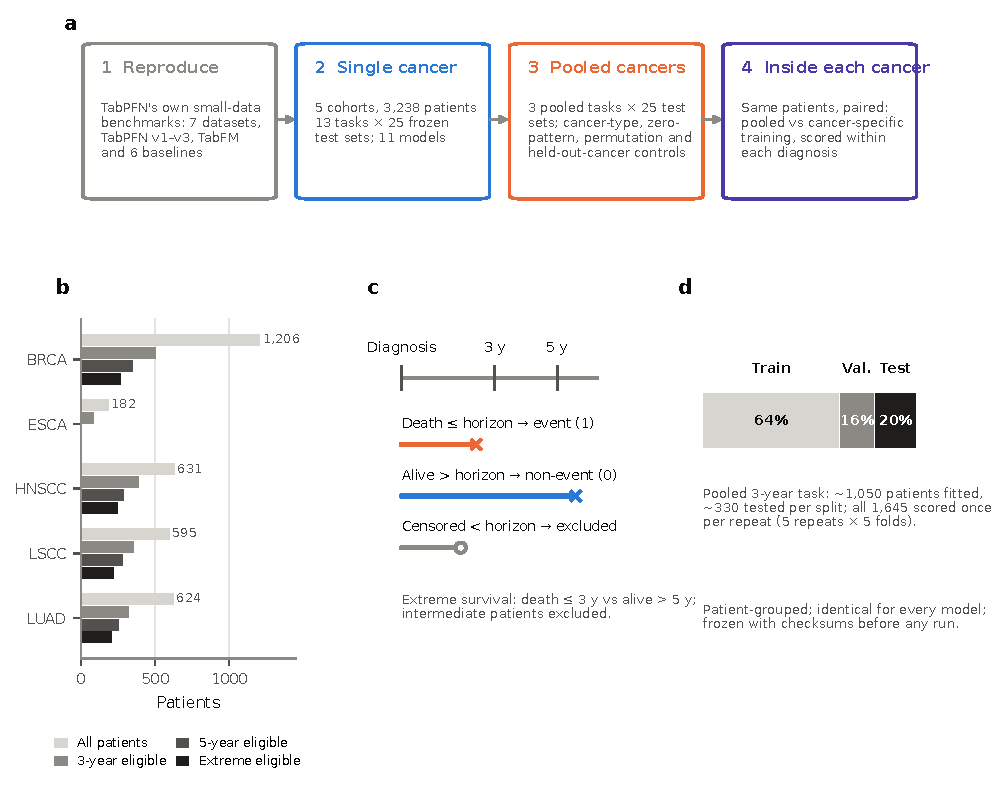
\includegraphics[width=\linewidth,height=0.64\textheight,keepaspectratio]{figures/reusability/fig1_roadmap_and_design.pdf}
\caption{\textbf{Study roadmap and evaluation design.} \textbf{a}, The four steps of the report: reproduction of TabPFN on its own benchmark datasets, evaluation within single cancers, evaluation on the pooled cancers with shortcut controls, and a paired return to within-cancer scoring. \textbf{b}, Patients per cohort: all patients (lightest bar) and those eligible for 3-year survival, 5-year survival and extreme survival (progressively darker bars); the number gives the cohort total. ESCA was too small to form the 5-year and extreme-survival endpoints. \textbf{c}, Fixed-horizon labels: death on or before the horizon is an event (1), follow-up beyond the horizon is a non-event (0), and patients censored before the horizon are excluded; extreme survival compares death within 3 years with survival beyond 5 years. \textbf{d}, Partition of patients in one frozen test set: about 64\% for training, where features are selected; 16\% for validation, used only to choose the decision threshold; and 20\% for testing, scored once. Splits are patient-grouped, identical for every model and frozen before any run.}
\label{fig:roadmap}
\end{figure}
